\documentclass[11pt, oneside]{article}   	% use "amsart" instead of "article" for AMSLaTeX format
\usepackage{geometry}                		% See geometry.pdf to learn the layout options. There are lots.
\geometry{letterpaper}                   		% ... or a4paper or a5paper or ... 
%\geometry{landscape}                		% Activate for for rotated page geometry
%\usepackage[parfill]{parskip}    		% Activate to begin paragraphs with an empty line rather than an indent
\usepackage{graphicx}				% Use pdf, png, jpg, or eps� with pdflatex; use eps in DVI mode
								% TeX will automatically convert eps --> pdf in pdflatex		
\usepackage{amssymb}
\usepackage{amsmath}
\usepackage{parskip}
\usepackage{color}
\usepackage{hyperref}

\title{Calculating a moment of inertia}
%\author{The Author}
%\section{}
%\subsection*{}
\date{}							% Activate to display a given date or no date

\graphicspath{{/Users/telliott_admin/Dropbox/Tex/png/}}
% \begin{center} 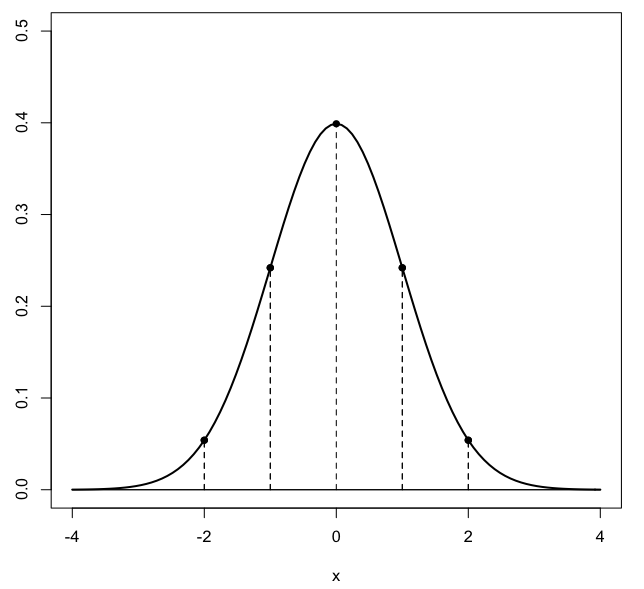
\includegraphics [scale=0.4] {gauss3.png} \end{center}
\begin{document}
\maketitle
\Large
The moment of inertia of a collection of discrete masses is the sum of each mass, times the square of the distance to the chosen axis of rotation.  
\subsection*{rods}
Imagine that we have a uniform (thin) rod, and it's going to rotate around the center of the rod.  Choose that as the origin of coordinates.  The ends of the rod are then at $-l/2$ and $+l/2$.

Calculate the mass per unit length $M/l$, and so in a tiny sliver of the rod of width $dx$, the mass at that position is $M/l \ dx$ and its moment is $Mx^2/l \ dx$.  We add them all up:
\[ I = \int_{-l/2}^{l/2} \frac{M}{l} x^2 \ dx \]
\[ =  \frac{M}{l} \ \frac{x^3}{3} \bigg |_{-l/2}^{l/2} = Ml^2 (\frac{1}{24} - - \frac{1}{24}) = \frac{1}{12} Ml^2 \]

If we move the axis to the end of the rod, then move the coordinate system as well, and we have
\[ \int_0^l \frac{M}{l} x^2 \ dx \]
\[ =  \frac{M}{l} \ \frac{x^3}{3} \bigg |_{0}^{l} = \frac{1}{3} Ml^2 \]  
There is a principle called the "parallel axis theorem" which says that 
\[ I = I_{CM} + md^2 \]
where $CM$ is the center of mass and $d$ is the distance between the two axes.  The first example was at the $CM$ of the rod, and the distance we moved was $l/2$ so we have
\[ I = \frac{1}{12} Ml^2 + M (\frac{l}{2})^2 = Ml^2 (\frac{1}{12} + \frac{1}{4}) = \frac{1}{3} Ml^2 \]

\subsection*{rings and disks}
Imagine the object is a ring, and we're rotating around the center.  Think of it as a sum of discrete pieces
\[ I = \sum_i m_i r^2 \]
But $r = R$ for every piece so we have
\[ I = R^2 \sum_i m_i = MR^2 \]
For a disk, we imagine adding up the contribution for a series of rings with increasing radius.  At radius $r$, the circumference of the ring is $2 \pi r$, and the area of the ring is $2 \pi r \ dr$.  The mass per unit area is $M/\pi R^2$ so the mass of each ring is
\[ m = \frac{M}{\pi R^2} \ 2 \pi r \ dr = \frac{2M}{R^2} r \ dr \]
Integrate mass times radius squared from $r=0 \rightarrow R$
\[ I = \int_0^R r^2 \frac{2M}{R^2} r \ dr \]
\[ = \frac{2M}{R^2} \ \frac{r^4}{4} \bigg |_{0}^{R} =  \frac{1}{2} MR^2 \]
Now, if we were to move the axis of rotation to the edge, we would have
\[ I = \frac{MR^2}{2} + MR^2 = \frac{3}{2} MR^2 \]
\subsection*{sphere}
Start with the sphere.  It's analogous to the ring, but harder.  I struggled with this one, by not using the appropriate slant height when calculating the area of a slice.  I found another approach online:

\small
\url{http://www.miniphysics.com/uy1-calculation-of-moment-of-inertia-of_04.html}
\Large

 \begin{center} 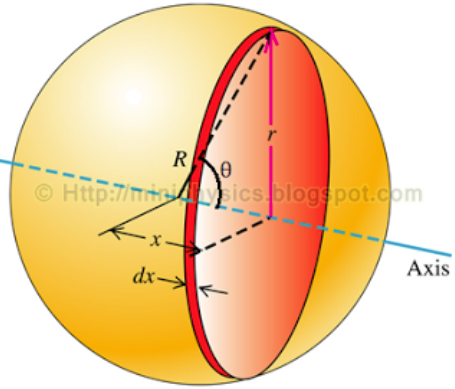
\includegraphics [scale=0.4] {moment_sphere.png} \end{center}

and I liked it so much I want to show that approach.  We slice the sphere perpendicular to the axis of rotation.  For each slice we have a ring of radius $r$ whose moment is
\[ dI = r^2 \ dm \]
where
\[ dm = \frac{M}{A} \ dA = \frac{M}{4\pi R^2} \ dA \]
The trick is to express the area of the ring (parametrize our slices) in terms of an angle $\theta$, shown in the figure ($\theta = 0 \rightarrow \pi$, where $\theta = \pi/2$ is perpendicular to the axis).  Doing this, we get the correct area for the width of the ring, namely $R \ d \theta$, and a total area for the ring of
\[ dA = 2 \pi r \ R \ d \theta \]
so
\[ dm =  \frac{M}{4\pi R^2} \ dA =   \frac{M}{4\pi R^2} \ 2 \pi r \ R \ d \theta =   \frac{M}{2 R} \ r \ d \theta \]
and then
\[ dI = r^2 \ dm =  \frac{M}{2 R} \ r^3 \ d \theta \]
Now, we need to get a relationship between $r$ and $\theta$, but from the diagram it's clear that
\[ r = R \sin \theta \]
so we have the integral
\[ I = \int dI = \frac{MR^2}{2}  \int_0^{\pi} \sin^3 \theta \ d \theta \]
This is pretty easy.  We do
\[ \sin^3 \theta \ d \theta = (1- \cos^2 \theta) \sin \theta \ d \theta \]
the integral is just
\[  \int \sin^3 \theta \ d \theta = - \cos \theta + \frac{\cos^3 \theta}{3} \ \bigg |_0^{\pi} = (1 - \frac{1}{3}) - (-1 + \frac{1}{3}) = \frac{4}{3} \]
and the answer is 
\[ \frac{2}{3} MR^2 \]

\subsection*{solid ball}
With the previous result in hand the solid ball is pretty easy.  We imagine a series of concentric spheres with increasing radius $r = 0 \rightarrow R$.  Each sphere has
\[ dI = \frac{2}{3} dm \ r^2 \]
\[ dm = \frac{M}{4/3 \pi R^3} \ 4 \pi r^2 = \frac{3M}{R^3} r^2 \]
so 
\[ dI = \frac{2M}{R^3} r^4 \]
\[ I = \int \ dI = \frac{2M}{R^3}  \int_0^R r^4 \]
\[ = \frac{2M}{R^3} \ \frac{R^5}{5} = \frac{2}{5} MR^2 \]

\subsection*{parallel axis theorem}
The proof of the parallel axis theorem is pretty easy (Fitzpatrick).  Choose the origin of coordinates to be at the center of mass of the body.  Orient the $z$-axis with the axis of rotation.  Orient the new axis so that the new moment of inertia lies along the $x$-axis at $x=d; y =0$.

Since the center of mass is at the origin
\[ \iiint x \ dx \ dy \ dz = 0 \]
with the integrals taken over the volume of the body.  The same is true for $y$ and $z$.

Now the square of the distance of any point in the body from the $z$-axis is $x^2 + y^2$, so the moment of inertion with respect to the center of mass is
\[ I_{CM} = M \frac{\iiint (x^2 + y^2) \ dx \ dy \ dz}{\iiint \ dx \ dy \ dz} \]

The new moment of inertia is
\[ I' = M \frac{\iiint ((x-d)^2 + y^2) \ dx \ dy \ dz}{\iiint \ dx \ dy \ dz} \]
Expanding and taking the constant $d$ outside the integral
\[ = M \frac{\iiint (x^2 + y^2) \ dx \ dy \ dz}{\iiint \ dx \ dy \ dz} - 2dM \frac{\iiint x \ dx \ dy \ dz}{\iiint \ dx \ dy \ dz} + d^2M \frac{\iiint \ dx \ dy \ dz}{\iiint \ dx \ dy \ dz}\]
The middle integral is zero and the first term is $I_{CM}$ so we have
\[ = I_{CM} + d^2M \frac{\iiint \ dx \ dy \ dz}{\iiint \ dx \ dy \ dz}\]
The third term is just $Md^2$
\[ I' = I_{CM} + Md^2 \]
I think this derivation assumes constant density, but it will still work with variable density, just add a function $\delta(x,y,z)$ which never has to be evaluated.

Just in case, let me show you Professor Shankar's version.  We will do this by summation, just pretend we are summing over lots of individual little mass elements with position vectors $\mathbf{r}_i$ from the center of mass.
\[ I_{CM} = \sum_i m_i |\mathbf{r}_i|^2 = \sum_i m_i (\mathbf{r}_i \cdot \mathbf{r}_i) \]
Now we move the axis of rotation to a new position with position vector $\mathbf{d}$ from the center of mass.  Notice that $\mathbf{d}$ will be the same for every $m_i$.  The new moment is
\[ I_{CM}' = \sum_i m_i (\mathbf{r}_i' \cdot \mathbf{r}_i') \] 
where
\[ \mathbf{d} +  \mathbf{r}_i'  = \mathbf{r}_i  \]
\[ \mathbf{r}_i' = \mathbf{r}_i - \mathbf{d} \]
and so
\[ \mathbf{r}_i' \cdot \mathbf{r}_i'  =  (\mathbf{r}_i - \mathbf{d}) \cdot (\mathbf{r}_i - \mathbf{d}) \]
\[ = \mathbf{r}_i \cdot \mathbf{r}_i - 2 \mathbf{r}_i \cdot  \mathbf{d} + \mathbf{d} \cdot \mathbf{d} \]
substitute into the moment calculation
\[ I_{CM}' = \sum_i m_i (\mathbf{r}_i \cdot \mathbf{r}_i) + \sum_i m_i |(-2) \mathbf{r}_i \cdot \mathbf{d} | + \sum_i m_i (\mathbf{d} \cdot \mathbf{d}) \] 
Now, the first term is $I_{CM}$, and in the third term, since $\mathbf{d}$ does not vary with $i$, it is just $d^2$ and we can pull it out of the sum
\[ I_{CM}' = I_{CM} + \sum_i m_i (-2)( \mathbf{r}_i \cdot \mathbf{d}) + d^2 \sum_i m_i \] 
\[ I_{CM}' = I_{CM} + \sum_i m_i (-2)( \mathbf{r}_i \cdot \mathbf{d}) + Md^2 \] 
We're almost there.  We need the middle term to vanish.The coordinates were set up so that $\mathbf{d}$ lies along the $x$-axis, so $ \mathbf{r}_i \cdot \mathbf{d}$ is just the constant $d$ times the $x$-component of $\mathbf{r}_i$ for each vector.
\[ \sum_i m_i (-2)( \mathbf{r}_i \cdot \mathbf{d})  = -2d \sum_i m_i  \mathbf{r}_{ix} \]
$\sum_i m_i  \mathbf{r}_{ix}$ is the $x$-component of the center of mass \emph{in this coordinate system}.  But we've chosen that point to be the origin.  So this term vanishes, leaving
\[ I_{CM}' = I_{CM} + Md^2 \] 

\end{document}  